% Sparsity pattern of the Jacobian d[x^d]P_7 / d alpha_i (rows: degree, columns: parameter).
% Characteristic-zero pattern: blue = nonzero constant, orange = nonconstant polynomial, white = zero.
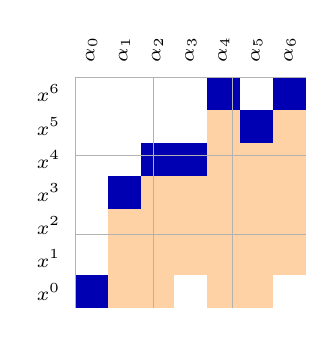
\begin{tikzpicture}[x=4.2mm, y=4.2mm, font=\scriptsize]
  \fill[fill=white] (0,0) rectangle (1,-1);
  \fill[fill=white] (1,0) rectangle (2,-1);
  \fill[fill=white] (2,0) rectangle (3,-1);
  \fill[fill=white] (3,0) rectangle (4,-1);
  \fill[fill=blue!70!black] (4,0) rectangle (5,-1);
  \fill[fill=white] (5,0) rectangle (6,-1);
  \fill[fill=blue!70!black] (6,0) rectangle (7,-1);
  \node[anchor=east] at (-0.15,-0.5) {$x^{6}$};
  \fill[fill=white] (0,-1) rectangle (1,-2);
  \fill[fill=white] (1,-1) rectangle (2,-2);
  \fill[fill=white] (2,-1) rectangle (3,-2);
  \fill[fill=white] (3,-1) rectangle (4,-2);
  \fill[fill=orange!35] (4,-1) rectangle (5,-2);
  \fill[fill=blue!70!black] (5,-1) rectangle (6,-2);
  \fill[fill=orange!35] (6,-1) rectangle (7,-2);
  \node[anchor=east] at (-0.15,-1.5) {$x^{5}$};
  \fill[fill=white] (0,-2) rectangle (1,-3);
  \fill[fill=white] (1,-2) rectangle (2,-3);
  \fill[fill=blue!70!black] (2,-2) rectangle (3,-3);
  \fill[fill=blue!70!black] (3,-2) rectangle (4,-3);
  \fill[fill=orange!35] (4,-2) rectangle (5,-3);
  \fill[fill=orange!35] (5,-2) rectangle (6,-3);
  \fill[fill=orange!35] (6,-2) rectangle (7,-3);
  \node[anchor=east] at (-0.15,-2.5) {$x^{4}$};
  \fill[fill=white] (0,-3) rectangle (1,-4);
  \fill[fill=blue!70!black] (1,-3) rectangle (2,-4);
  \fill[fill=orange!35] (2,-3) rectangle (3,-4);
  \fill[fill=orange!35] (3,-3) rectangle (4,-4);
  \fill[fill=orange!35] (4,-3) rectangle (5,-4);
  \fill[fill=orange!35] (5,-3) rectangle (6,-4);
  \fill[fill=orange!35] (6,-3) rectangle (7,-4);
  \node[anchor=east] at (-0.15,-3.5) {$x^{3}$};
  \fill[fill=white] (0,-4) rectangle (1,-5);
  \fill[fill=orange!35] (1,-4) rectangle (2,-5);
  \fill[fill=orange!35] (2,-4) rectangle (3,-5);
  \fill[fill=orange!35] (3,-4) rectangle (4,-5);
  \fill[fill=orange!35] (4,-4) rectangle (5,-5);
  \fill[fill=orange!35] (5,-4) rectangle (6,-5);
  \fill[fill=orange!35] (6,-4) rectangle (7,-5);
  \node[anchor=east] at (-0.15,-4.5) {$x^{2}$};
  \fill[fill=white] (0,-5) rectangle (1,-6);
  \fill[fill=orange!35] (1,-5) rectangle (2,-6);
  \fill[fill=orange!35] (2,-5) rectangle (3,-6);
  \fill[fill=orange!35] (3,-5) rectangle (4,-6);
  \fill[fill=orange!35] (4,-5) rectangle (5,-6);
  \fill[fill=orange!35] (5,-5) rectangle (6,-6);
  \fill[fill=orange!35] (6,-5) rectangle (7,-6);
  \node[anchor=east] at (-0.15,-5.5) {$x^{1}$};
  \fill[fill=blue!70!black] (0,-6) rectangle (1,-7);
  \fill[fill=orange!35] (1,-6) rectangle (2,-7);
  \fill[fill=orange!35] (2,-6) rectangle (3,-7);
  \fill[fill=white] (3,-6) rectangle (4,-7);
  \fill[fill=orange!35] (4,-6) rectangle (5,-7);
  \fill[fill=orange!35] (5,-6) rectangle (6,-7);
  \fill[fill=white] (6,-6) rectangle (7,-7);
  \node[anchor=east] at (-0.15,-6.5) {$x^{0}$};
  \draw[gray!60, very thin] (0,0) grid (7,-7);
  \node[anchor=west, rotate=90] at (0.5,0.15) {$\alpha_{0}$};
  \node[anchor=west, rotate=90] at (1.5,0.15) {$\alpha_{1}$};
  \node[anchor=west, rotate=90] at (2.5,0.15) {$\alpha_{2}$};
  \node[anchor=west, rotate=90] at (3.5,0.15) {$\alpha_{3}$};
  \node[anchor=west, rotate=90] at (4.5,0.15) {$\alpha_{4}$};
  \node[anchor=west, rotate=90] at (5.5,0.15) {$\alpha_{5}$};
  \node[anchor=west, rotate=90] at (6.5,0.15) {$\alpha_{6}$};
\end{tikzpicture}
